\documentclass[tikz,border=6pt]{standalone}
\usepackage{amsmath,amssymb}
\usepackage{xcolor}
\definecolor{accent}{HTML}{A13D2C}
\definecolor{accent2}{HTML}{2B5F6B}
\definecolor{muted}{HTML}{5A564F}
\definecolor{panel}{HTML}{F8F6F0}
\definecolor{linecol}{HTML}{D8D2C4}
\definecolor{astroblue}{HTML}{1B4F72}
\definecolor{sunyellow}{HTML}{E8A33D}
\definecolor{colthree}{RGB}{60,140,80}
\usetikzlibrary{calc,arrows.meta}
\usepackage[T1]{fontenc}\usepackage{newpxtext,newpxmath}  % same fonts as the notes
\begin{document}
% Thin-disk temperature T/T_* = (R_in/r)^{3/4} (1 - sqrt(R_in/r))^{1/4}, and the asymptote (R_in/r)^{3/4}, on log axes; r/R_in from 1 to 10^3.
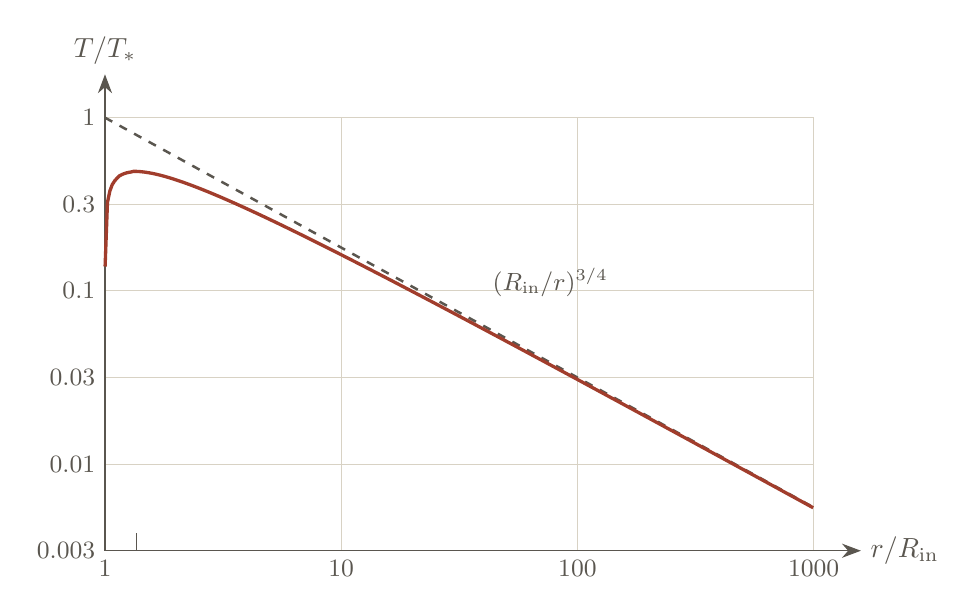
\begin{tikzpicture}[x=3cm,y=2.2cm, >={Stealth[length=2.4mm]}]
  \draw[linecol] (0,-2.5) grid[xstep=1,ystep=0.5] (3,0);
  \draw[->, muted] (0,-2.5) -- (3.2,-2.5) node[right] {$r/R_{\rm in}$};
  \draw[->, muted] (0,-2.5) -- (0,0.25) node[above] {$T/T_*$};
  \foreach \x/\l in {0/1,1/10,2/100,3/1000} \node[below, muted] at (\x,-2.5) {\small \l};
  \foreach \y/\l in {0/1,-0.5/0.3,-1/0.1,-1.5/0.03,-2/0.01,-2.5/0.003} \node[left, muted] at (0,\y) {\small \l};
  \draw[dashed, muted, line width=0.9pt, domain=0:3, samples=50] plot (\x, {-0.75*\x});
  \draw[accent, line width=1.2pt, domain=0.0005:3, samples=300] plot (\x, {-0.75*\x + 0.25*log10(1 - exp(-0.5*\x*2.302585))});
  \draw[muted] ({log10(49/36)},-2.5) -- ({log10(49/36)},-2.4);
  \node[muted, right] at (1.6,-0.95) {\small $(R_{\rm in}/r)^{3/4}$};
\end{tikzpicture}
\end{document}
